\documentclass[10pt]{beamer}
\usetheme{metropolis}

\usepackage{amsmath, booktabs, fontawesome5, natbib, subfigure, xcolor}

\usepackage[font=small,skip=0pt]{caption}

\usepackage{pgfplots}
\usepgfplotslibrary{dateplot}

\usepackage{xspace}
\newcommand{\themename}{\textbf{\textsc{metropolis}}\xspace}

\usepackage{graphicx}
\graphicspath{{../imgs/}}

\usepackage[T1]{fontenc}
\usepackage[french]{babel}

\usepackage{appendixnumberbeamer}

\usepackage{tikz}
\usetikzlibrary{shapes.geometric, arrows}
\tikzstyle{rect} = [rectangle, rounded corners, minimum width=2cm, minimum height=1.5cm, text centered, draw=black, fill=black!30]
\tikzstyle{squa} = [square, rounded corners, minimum width=1.25cm, minimum height=1.25cm, text centered, draw=black, fill=black!30]
\tikzstyle{elli} = [ellipse, minimum width=1.25cm, minimum height=1cm, text centered, draw=black, fill=black!30]
\tikzstyle{circ} = [circle, minimum width=1cm, minimum height=1cm, text centered, draw=black, fill=black!30]
\tikzstyle{arrow} = [thick,->,>=stealth]
\tikzstyle{drrow} = [thick,<->,>=stealth]
\tikzstyle{dline} = [dashed, ->, >=stealth]
\tikzstyle{dotted} = [densely dotted, ->, >=stealth]

\def\firstcircle{(90:1.75cm) circle (2.5cm)}
\def\secondcircle{(210:1.75cm) circle (2.5cm)}
\def\thirdcircle{(330:1.75cm) circle (2.5cm)}
\tikzset{fontscale/.style = {font=\relsize{#1}}}

\titlegraphic{\hfill\includegraphics[height=1.25cm]{~/Documents/scpobx/logo.pdf}}
\title{Méthodes des sciences sociales}
\subtitle{Séance 2: Le projet de recherche}
\author{Mickael Temporão}
\institute{\faTwitter~$@$mickaeltemporao}
\date{}

\begin{document}

\maketitle

\begin{frame}{Méthodes des sciences sociales}
    \onslide<1->{
        \begin{block}{Ordre du jour}
            \begin{itemize}
                \item Présentation et discussion
                \item La méthode scientifique
                \item Le projet de recherche
            \end{itemize}
        \end{block}
    }
    \vspace{24pt}
    \onslide<2->{
        \begin{block}{\faTrophy~BONUS}
        \begin{itemize}
            \item[] \faGithubSquare~Github
            \item[] \faMarkdown~Markdown
        \end{itemize}
        \end{block}
    }
\end{frame}

\begin{frame}{\faExclamationTriangle~RAPPEL}
        \begin{block}{\faSlack~Slack}
            \begin{itemize}[<+->]
                \item Installez l'application sur \faLaptop~et/ou \faMobile
                \item Si \faAt, alors \faReply
                \item Soyez actifs sur les \faHashtag channels
            \end{itemize}
        \end{block}
    \onslide<4->{
        \begin{block}{\faTools~Cours \& Outils}
            \begin{itemize}[<+->]
                \item Utilisez ces outils dans d'autres contextes
                \item Posez des questions sur les possibilités
                \item Demandez de l'aide si vous êtes bloqués
            \end{itemize}
        \end{block}
    }
\end{frame}

\section{La méthode scientifique}


\begin{frame}{La méthode scientifique}
    \onslide<1-> {
        \begin{block}{Qu'est-ce que la science?}
            \begin{itemize}
                \item <2-> Un pratique utilisant une méthode systématique d'observation de phénomènes dans le but d'accroitre notre connaissance sur un sujet.
                \item <3-> La méthode systématique = la méthode scientifique.
            \end{itemize}
        \end{block}
    }
    \onslide<4-> {
        \begin{block}{Trois étapes}
            \begin{enumerate}
                \item <5-> Question initiale sur un phénomène
                \item <5-> Développement d'une théorie proposant une réponse à la question
                \item <5-> Collecte des données empiriques pour tester la théorie
                    \begin{itemize}
                        \item Les données sont collectés de manière systématique!
                    \end{itemize}
            \end{enumerate}
        \end{block}
    }
    \onslide<6-> La méthode scientifique s'ancre dans le courant \textbf{positiviste}!
\end{frame}

\begin{frame}{Le positivisme}
    \onslide<1-> {
        \begin{columns}
            \begin{column}{.7\textwidth}
                \onslide<2>{
                \begin{itemize}
                    \item Introduit par Auguste Compte
                    \item Les phénomènes peuvent être étudiés en les observant.
                    \item Ces observations peuvent être regroupées afin d'obtenir des faits et créer théories qui peuvent nous aider à comprendre le monde.
                \end{itemize}
            }
            \end{column}
            \begin{column}{.3\textwidth}
            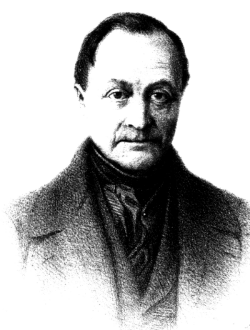
\includegraphics[width=\textwidth]{comte}
            \end{column}
        \end{columns}
    }
\end{frame}


\begin{frame}{C'est quoi le positivisme?}
        \begin{columns}
            \begin{column}{.7\textwidth}
                \onslide<2-> {
                \begin{block}{Positif?}
                    \onslide<3-> {
                    Une théorie positiviste est une théorie qui est objective et basée sur des faits.
                }
                \end{block}
            }
                \onslide<4-> {
                \begin{block}{Normatif}
                \onslide<4-> {
                    Une théorie normative est une théorie qui est basée sur des jugements de valeurs et des interprétations.
                }
                \end{block}
        }
            \end{column}
            \begin{column}{.3\textwidth}
            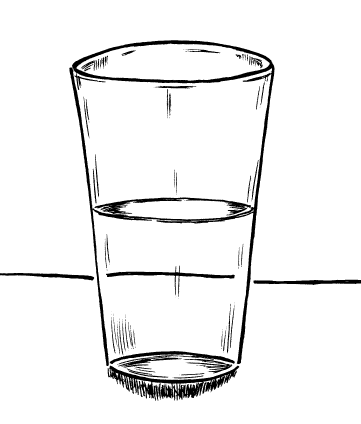
\includegraphics[width=\textwidth]{glass}
            \end{column}
        \end{columns}
\end{frame}


\begin{frame}{La sociologie positiviste}
    \begin{block}{L'étude de la société basé sur l'observation systématique de comportements sociaux}
    \end{block}
    \begin{itemize}
        \item Importance de l'objectivité!
        \item Mettre de côté ses valeurs et croyances
        \item Approcher son objet d'étude comme un observateur neutre
        \item Se baser sur des preuves empiriques pour répondre à des questions sur le fonctionnement du monde social.
    \end{itemize}

    \onslide<2->{
    \begin{block}{Quel types de preuves empiriques?}
    \begin{itemize}
        \item<3-> Données quantitatives
        \item<3-> Données qualitatives
    \end{itemize}
    \end{block}
}
\end{frame}

\section{Application}
\begin{frame}{Le projet de recherche}
    \begin{block}{Exercice}
    \begin{enumerate}
        \item Identifiez un sujet
        \item Recherchez des articles scientifiques sur le sujet
        \item Repérez les questions auxquelles s'intéressent les auteurs
        \item Développez une question de recherche
        \item<2>[\faArrowRight~]\textbf{Présentez!}
    \end{enumerate}
    \end{block}
\end{frame}

\section{Technique}

\maketitle

\end{document}
